\documentclass[11pt]{article}

\usepackage{amsmath,amssymb,epsfig}
\usepackage[T1]{fontenc}
\usepackage{ae,aecompl}
\usepackage{epsfig}
\usepackage{subfigure}
\addtolength{\voffset}{-1cm}
\addtolength{\hoffset}{-1cm}
\setlength{\parindent}{0in}
\addtolength{\textwidth}{1.8cm}
\addtolength{\textheight}{1cm}
\addtolength{\parskip}{.5cm}

% Example definitions.
% --------------------
\def\e{{e^{j\omega}}}
\def\W{{W_M}}
\def\sumk{{\sum_{k=-\infty}^{\infty}}}
\def\x{{\mathbf x}}
\def\X{{\mathbf X}}
\def\Y{{\mathbf Y}}
\def\u{{\mathbf u}}
\def\U{{\mathbf U}}
\def\x{{\mathbf x}}
\def\s{{\mathbf s}}
\def\A{{\mathbf A}}
\def\y{{\mathbf y}}
\def\w{{\mathbf w}}
\def\B{{\mathbf B}}
\def\a{{\mathbf a}}
\def\D{{\mathbf D}}
\def\P{{\mathbf P}}
\def\n{{\mathbf n}}
\def\V{{\mathbf V}}
\def\R{{\mathbf R}}
\def\I{{\mathbf I}}
\def\M{{\mathbf M}}
\def\sech{{\mathrm{sech}}}
\def\L{{\cal L}}
\def\Cum{{\rm{Cum}}}
\def\var{{\rm{var}}}
\def\T{{\mathbf T}}
\def\C{{\mathbf C}}
\def\tf{{\emph{t-f}}}


% Title.
% ------
\title{\large{\textbf{SGN-1156 SIGNAL PROCESSING TECHNIQUES}}}
\author{Exercise 1}
%\author{\textbf{Assistant:}\\
%Germ{\'a}n G{\'o}mez-Herrero\\
%german.gomezherrero@tut.fi\\
%Room TE414}
%
% Author and date.
% ---------------
\date{2009 Fall}



\begin{document}

\maketitle


\textbf{PROBLEM 1:}  Consider a system with the following input-output relationship:

\[
y[n] = \frac{1}{x[n]}+x[n-1]
\]

where $x[n]$ is the input to the system and $y[n]$ is the system's output. Is this system linear? Is it time-invariant? Is it stable?. Could you determine the ouput of the system to an arbitrary input by using only the system's impulse response?. Justify your answers. 

\vspace{1cm}



\textbf{PROBLEM 2:} Consider a system with the following input-output relationship:

\[
y[n] = (n-1)^2 x[n]
\]

where $x[n]$ is the input to the system and $y[n]$ is the system's output. Is this system linear? Is it time-invariant? Is it causal? Is it stable?

\vspace{1cm}




\textbf{PROBLEM 3:} Consider a system with the following input-output relationship:

\[
y[n] = x[n]+2x[n-5]
\]

where $x[n]$ is the input to the system and $y[n]$ is the system's output. Is this system stable?

\vspace{1cm}



\textbf{PROBLEM 4 (problem 2.64 from the book):}  Determine the expression for the impulse response of the LTI system in the figure below.


\begin{figure}[h!]
	\centering
		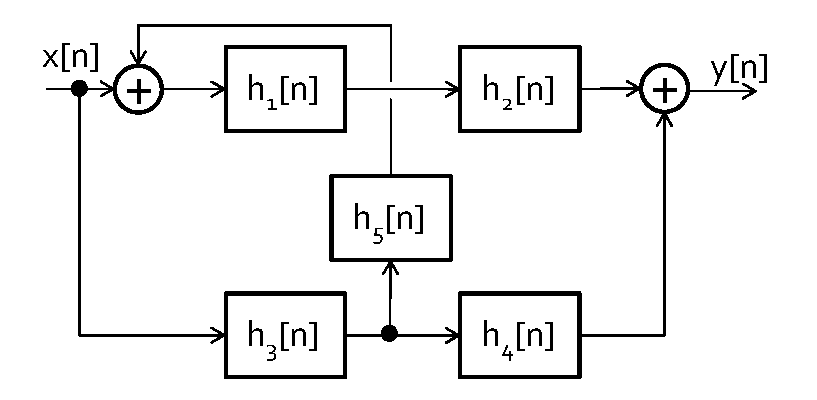
\includegraphics[width=.75\textwidth]{./system.eps}
	%\caption{dagd}
	%\label{fig:system}
\end{figure}



\vspace{1cm}

\textbf{PROBLEM 5 (problem 2.48 from the book):} A periodic sequence $\tilde{x}[n]$ with a period $N$ is applied as an input to an LTI discrete-time system characterized by an impulse response $h[n]$ generating an output $y[n]$. Is $y[n]$ a periodic sequence? If it is, what is its period?






\end{document}